\chapter{序論}
\label{chap:introduction}

\section{背景}
%目的に書いたことをこっちに持ってくる
近年,スマートフォンの急速な普及により数多くのアプリケーションが開発され,人々が毎日利用している,そのアプリケーションの開発には人々が感じている課題の洗い出し,適切な仕様の確定,使いやすいインタフェースの設計,実装など専門的で複雑な工程が多数存在する.中でもインタフェース設計とその実装は開発全体の中で設計段階で45%,実装段階で50%,保守段階で37%の時間を占めると言われている\cite{myers1992survey}.

またデザインカンパニーであるGoodpatchの社長である土屋は創業の原点について次のように述べており,デザインの重要性について述べている.

%goodpatchを持って来ずに一般的なものを持ってくる
\begin{quotation}
Goodpatchは2011年にUIデザインに特化したデザイン会社としてスタートしました。2011年に起業前に渡ったサンフランシスコでは創業期のInstagramやUber、Airbnbなど多くのスタートアップの共同創業者にデザイナーがおり、ベータ版からUIデザインに力を入れ、ユーザー体験を最初から考え、デザインを重要な差別化要素としてプロダクト開発を行っておりました。日本の環境と大きなギャップを感じた土屋は日本に帰り、創業したことがGoodpatchの原点です。\cite{goodpatchwhydesign}
\end{quotation}

大手企業の大規模開発では社内に専門知識を持ったデザイナが在籍していたり,Goodpatchのようなデザインカンパニーと共に設計を行うことが可能であるが専門のデザイナが在籍しないスタートアップ企業やインディーズ開発,個人開発ではこれらを行うのは非常に困難である.

%Garretの説明をする.
また,日本ではデザインが装飾などの表層的なもののみを指すと誤解されていると指摘されている\cite{goodpatchwhydesign}.本来のデザインの役割とは,プロダクトの本質的な価値を見出し,価値を最大化させることである.James GarretのUX五段階モデル(図\ref{fig:garretuxmodel})は,具象と抽象を行き来しながら,戦略,要件,構造,骨格,表層全てを設計することがデザインであると示している.

\begin{figure}[htbp]
  \begin{minipage}{\hsize}
    \begin{center}
       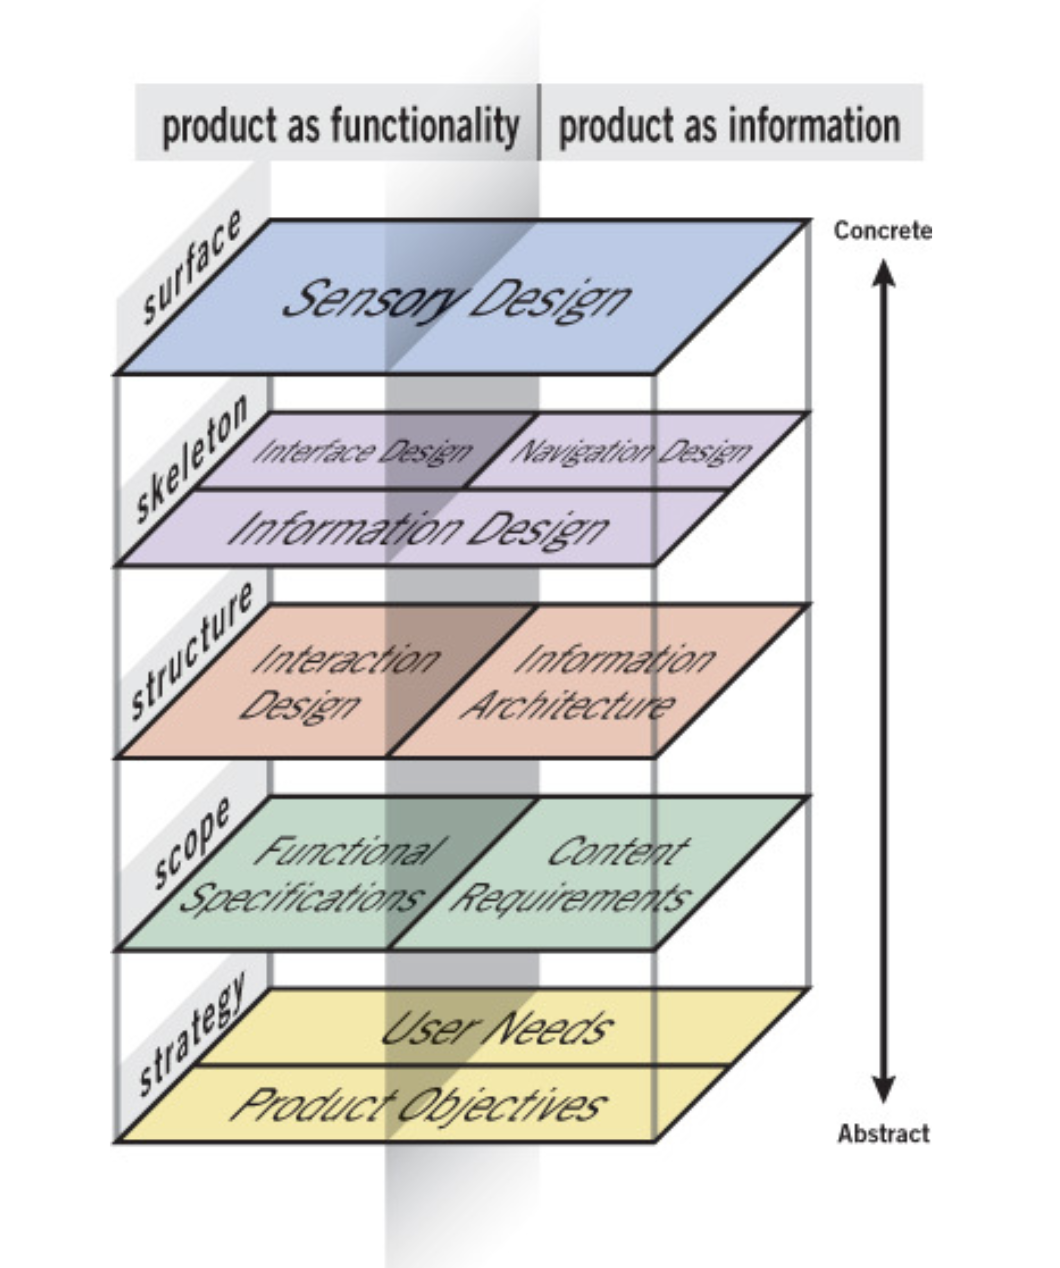
\includegraphics[width=100mm]{img/uxmodel.png}
    \end{center}
    \caption{GarretのUX五段階モデル\cite{garrett2010elements}}
    \label{fig:garretuxmodel}
  \end{minipage}
\end{figure}

%サブセクションが内容を表していなかったので変えた
\subsection{システム開発におけるデザイナの役割と現状}

%↓尾崎氏の個人的意見になっているので客観的に

資金や人的リソースが十分な大規模開発では役割としてのデザイナが参画している場合も多いが,前述のようなデザインの能力を有しているとは限らない.職業としてのデザイナを職業としている人の中でもGarretが述べている本来のデザインを忘れ,表層のデザインに注力してる場合が多く本来のデザインが一般に普及しているとは言えない.(←ソースは?

また,デザイナよりもアプリに向き合っている時間が長いエンジニアの方がアプリのデザインについて専門的知識を持ち開発をおこなっている場合も多数ある.エンジニアの場合GarretのUX五段階モデルもさることながら,UIが実際に動く仕組みを理解している分,内部構造という面での専門知識を有してる場合も多い.
実際に日本経済新聞電子版のメンバーによるデザインに関する登壇では14個中全ての登壇がエンジニア,又はエンジニア経験のある人の登壇となっている.\cite{nikkeislide}

個人開発アプリは大規模開発するほど収益が見込まれないものの,ニッチな消費者のニーズにあうさまざまなアプリケーションがアプリストアにリリースされている.しかしながら資金,時間,人的リソースが十分にない個人開発では開発者がデザインの重要性について理解した専門家がいないことにより使い勝手が悪いものや,表層のデザインにのみ注力したアプリケーションがあり,消費者のニーズに答えられずにいる.

%以上のことから下の(1)(2)が導かれていない.上で言っているのはエンジニアが専門知識を有しているので大規模開発ではエンジニアがデザインをすればいい,個人開発では専門家が居ないと言っているだけなので(1)を導くには飛躍しすぎている.

%(2)については奥深くのデザインが何なのかわからない.

以上のことから,(1)現在は大規模な開発でしか行われていない専門性の高いユーザインタフェースデザインのハードルを下げること,(2)表層のデザインにとらわれずに奥深くのデザインに注力することができる手法を開発することが求められる.

\section{目的}
本研究では(1)現在は大規模な開発でしか行われていない専門性の高いユーザインタフェースデザインのハードルを下げ,(2) 表層のデザインにとらわれずに奥深くのデザインに注力することができるようにするシステムの開発を目指す.

%↓本当か?設計手法はいくつかあるのでは?OOUIとか.それらの不満点を示す必要がある.UI設計の手法を確立すれば自動生成できるというのはおかしくない?別の話では?「本来のデザイン」がよくわからない.

現在のUIデザインには確立された設計手法はなく,デザイナの経験やセンスに頼っているものの,既存のUIを分析することによりUI設計の手法を確立すれば簡易なUI自動生成システムになり得る.また,(2)注力されがちであった表層のデザインを自動化することでデザイナ,個人開発者が本来のデザインに向き合うことにも目を自然と向けられるようになることが可能になる.

本研究ではこの手法になりうる仮説として,1画面に必要な要素一覧,各要素の相対的な優先度,要素同士のグルーピングからUIを自動で生成する手法を提案する.%ここでノーデザインという言葉を主張していく

そして提案した手法をもとに1画面に必要な要素一覧,各要素の相対的な優先度,要素同士のグルーピングの情報からiOSネイティブアプリケーショ
ンのソースコード(SwiftUI)を自動で生成するシステムを開発した.そして,開発したシステムの有用性を示した.
\section{問題の所在}

\begin{itemize}
	\item 質の高いUIを設計するには専門知識が求められる.
	\item デザインを表層のグラフィックデザインだけだと誤解している場合が多く,専門知識の欠如に関する自覚が薄い.
	\item 既存のノーコードではデザインは自分で行う又はテンプレートから選んだデザインを使用する必要がある
	\item ノーコードでは生成される成果物がアプリケーションのソースコードではないため.ノーコードでできる範囲を超えた機能の実装は困難である.
	\item 機械学習を用いた自動生成では一意性が担保できない.
	\item GANで生成したUIは画像なのでアプリとして機能しない.
\end{itemize}
また,スマートフォンのUIは2007年の初代iPhoneから,パソコンについては1984年の初代Macintoshから基本的なUIは全く変わっていないにもかかわらず,UIの生成の法則性の研究はあまり行われてこなかった.
以上のことから表層のデザインを自動化し,専門知識のない人でも質の高いUIを構築できるシステムの開発が求められる.


\section{本論文の構成}

本論文の構成を示す.

第\ref{chap:introduction}章では本研究の背景について述べた.第\ref{chap:auto-gen}章では要素,優先度,グルーピングからUIを自動生成する手法を提案し,第\ref{chap:impl}章ではその手法をもとにiOS向けネイティブアプリケーションのコードを生成するシステムを提案する.そして,それらの有効性を示す.第\ref{chap:conclusion}章の結論では本研究を総括し,考察と展望を述べる.そして最後に第\ref{chap:prevresearch}章では関連研究と関連プロダクトを整理する.付録として,本研究で行った実験で得られたデータを添付する.
